\section{Part 6}
Example 8.12 was simulated to plot the distribution of the p-values generated from the one sample \textit{t} testing. Figure \ref{fig:part6} was reproduced below with the following snippet:

\begin{lstlisting}
    NUMSAMPS <- 10000

    # initialize distribution variables
    generateHist <- function(mu, filename) {

        # initialize empty arrays
        sampPScores <- generatedData <- rep(0, times=NUMSAMPS)

        # generate 10000 samples
        for (i in 1:NUMSAMPS) {

            generatedData <- rnorm(4, 20, 2)

            # store the sample means in vector
            xbar <- mean(generatedData)
            s <- sd(generatedData)

            tScore <- (xbar - mu)/(s/2)
            sampPScores[i] = pt(tScore, df=3)

        }

        # generate density histograms to display percentage
        h <- hist(
            sampPScores
        )
        h$density = h$counts/sum(h$counts)*100

        # dump plots into PNG
        png(
            filename=paste0("figures/", filename), 
            units="in", width=4, height=4, res=200
        )
        plot(
            h, freq=FALSE,
            main=NULL,
            xlab="P-value",
            ylab="Percent"
        )
        dev.off()

    }

    generateHist(mu=20, filename="part6a.png")
    generateHist(mu=21, filename="part6b.png")
    generateHist(mu=22, filename="part6c.png")
\end{lstlisting}

    \begin{figure}[ht]
        \centering

        \begin{subfigure}[b]{0.5\linewidth}
            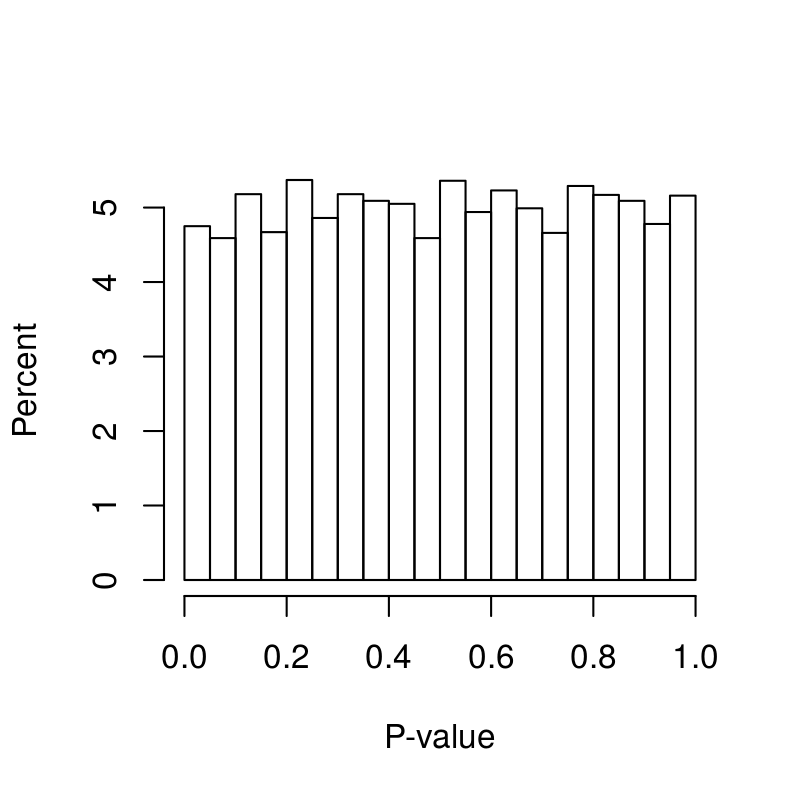
\includegraphics[width=0.9\textwidth]{figures/part6a.png}
            \caption{$\mu=20$}
        \end{subfigure}
        \begin{subfigure}[b]{0.5\linewidth}
            \centering
            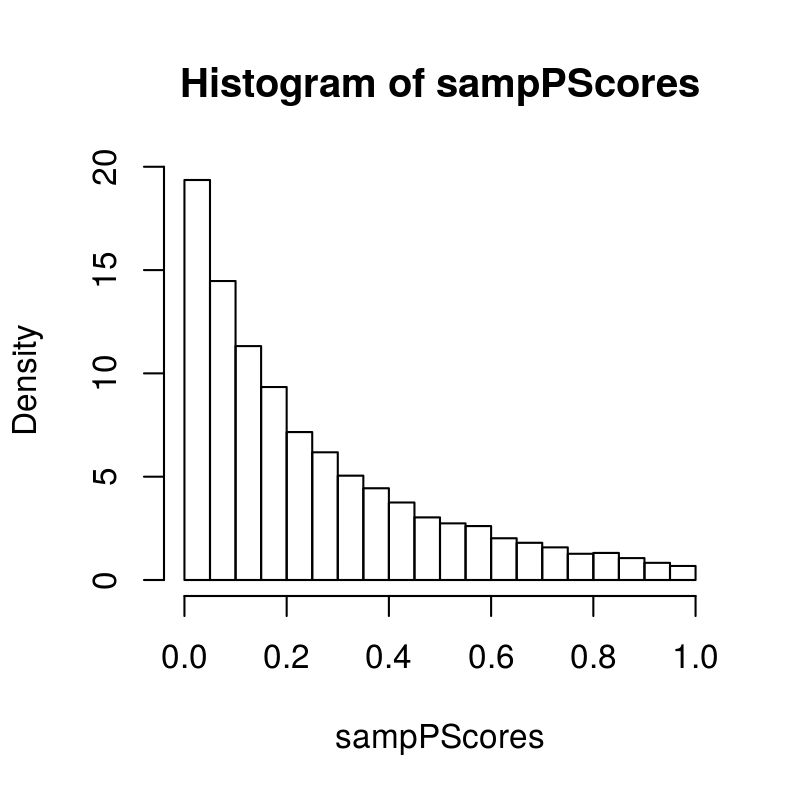
\includegraphics[width=0.9\textwidth]{figures/part6b.png} % first figure itself
            \caption{$\mu=21$}
        \end{subfigure}\hfill
        \begin{subfigure}[b]{0.5\linewidth}
            \centering
            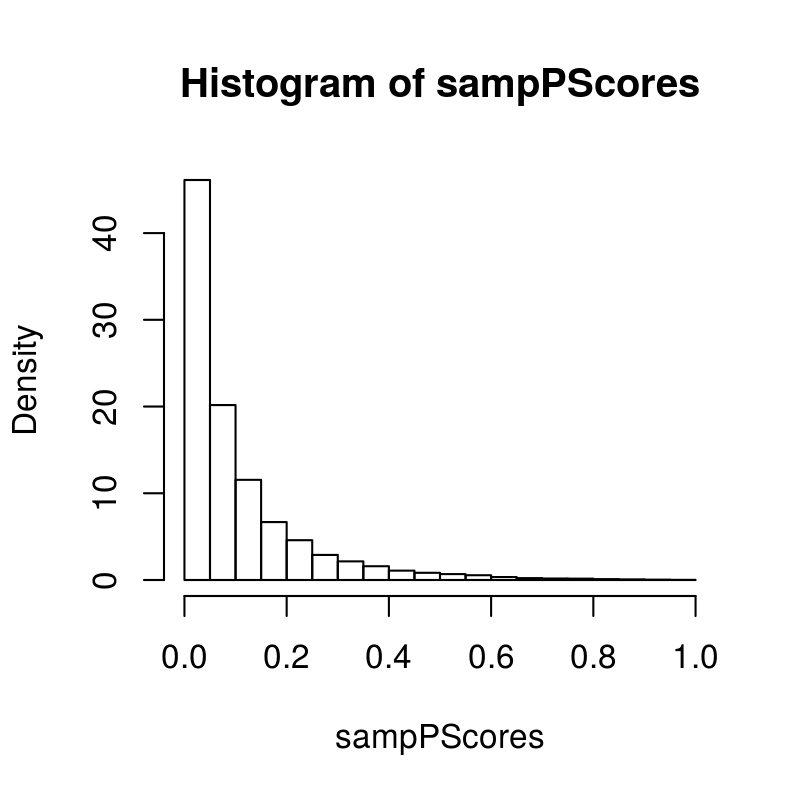
\includegraphics[width=0.9\textwidth]{figures/part6c.png} % second figure itself
            \caption{$\mu=22$}
        \end{subfigure}
        \caption{P-value Simulations for Example 8.12}
    \end{figure} \label{fig:part6}
